
\chapter{Computação em Nuvem} \label{cap2}

O objetivo deste capítulo é mostrar os conceitos envolvidos no paradigma de computação distribuída, mais especificamente os de Computação em Nuvem, abordando suas características e suas particularidades. Também descreve as chamadas Federações de Nuvens Computacionais e como este trabalho pretende utilizá-las para integrar um Sistema Gerenciador de Workflows Científicos à atual plataforma do BioNimbuZ. Para isso, a Seção \ref{cap2sec1} mostra o histórico da computação distribuída e seus principais elementos (como Grids e Clusters), a Seção \ref{cap2sec2} apresenta os conceitos básicos que norteiam o entendimento sobre nuvens computacionais, mostrando como diversas pesquisas contribuíram para o conceito atual desta tecnologia. A Seção \ref{cap2sec3} mostra os detalhes da chamada Federação de Nuvens Computacionais, quais seus objetivos, suas características e o que a distingue dos outros modelos de computação distribuídas. A Seção \ref{cap2sec4} mostra o conceito de um Workflow Científico e a Seção \ref{cap2sec5} descreve o que é um Sistema Gerenciador de Workflows Científicos.

\section{Sistemas Distribuídos} \label{cap2sec1}

A Internet é utilizada por bilhões de pessoas com vários propósitos diferentes, como ler e-mails, visualizar conteúdo multimídia, fazer compras ou apenas realizar uma busca por um assunto de interesse. Isso passa ao usuário a ilusão de que a informação e o sistema que a provê se encontram localmente em sua máquina. Mas, a internet representa um enorme sistema distribuído que se parece como um recurso único disponível em com um conjunto mínimo de configuração de conexão e em apenas poucos cliques [1].

O conceito de sistema distribuído possui diversas definições e pontos de vista. Colouris define um sistema distribuído como “um sistema em que componentes de hardware e software comunicam e coordenam suas ações apenas trocando mensagens” [7]; Tanenbaum o define como “uma coleção de computadores independentes que aparecem ao usuário do sistema como um único computador” [8]; Keith Marzullo [9] define um sistema distribuído da seguinte maneira: “Um sistema distribuído é uma coleção de processos sequenciais $P_1, P_2, ..., P_n$ e uma rede capaz de implementar canais de comunicação unidirecionais entre pares de processos para troca de mensagem”. 

Um dos aspectos mais importantes de sistemas distribuídos é a transparência. Esse conceito
Pelas definições, é possível elencar alguns aspectos comuns e essenciais que nos ajuda a distinguir sistemas distribuídos: 

\begin{itemize}
    \item São formados por um conjunto de computadores (ou unidades de processamento);
    \item São conectados por uma rede, sua comunicação é feita através de troca de mensagens, portanto não compartilham memória;
    \item São vistos pelo usuários como um recurso único (transparência [8]);
    \item Facilitam a utilização de recursos por usuários (ou aplicações).
    \item São escaláveis, isto é, possibilitam o aumento ou a diminuição de usuários ou recursos de maneira facilitada.
    \item Possuem desafios de temporização e sincronização.
    Assim, embora seja possível perceber os desafios inerentes à implementação deste tipo de sistema, o ganho de poder computacional vale à pena esse esforço.
\end{itemize}

\subsection{Cluster Computacional} \label{cap2sec1subsec1}

A primeira iniciativa na construção do conceito e implementação de Clusters Computacionais foi realizada pela IBM em meados dos anos 60 como alternativa de interligar grandes Mainframes para prover aos seus usuários uma forma comercial mais eficiente de paralelismo. Contudo, o conceito de Clusterização não ascendeu como previsto até o surgimento de outras três tecnologias: microprocessadores de alta-performance, redes de alta velocidade e protocolos para computação distribuída de alta-performance [13]. Os recentes avanços nessa tecnologias, somadas à sua acessibilidade (baixo preço decorrente da alta demanda) facilitaram a implementação de clusters computacionais como solução do antigo problema da eficiência de custos na busca de sistemas paralelos de alta performance.

\begin{figure}[h!]
\centering
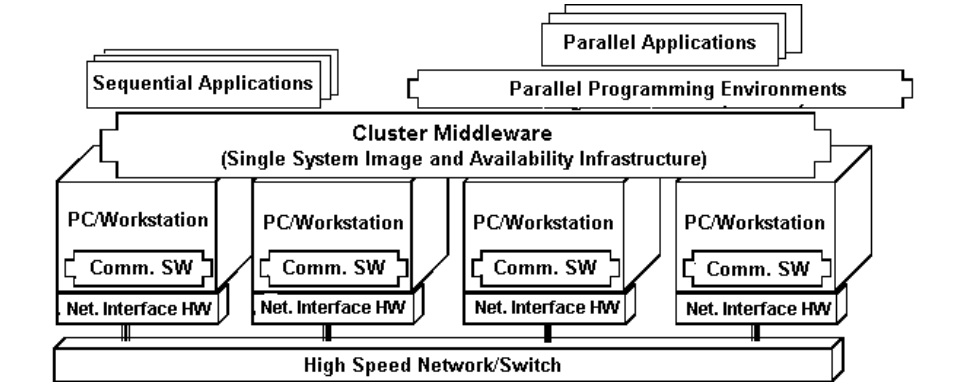
\includegraphics[scale=0.61]{images/cluster_architecture.jpg}
\caption{Arquitetura de um Cluster}
\label{fig:cluster_architecture}
\end{figure}

Abaixo estão listados alguns componentes essenciais em computadores utilizados em clusters [14]:

\begin{itemize}
    \item Vários computadores de alta performance (PCs, Workstations, Mainframes).
    \item Sistemas Operacionais.
    \item Conectados por uma rede de alta performance (como Gigabit Ethernet).
    \item Middleware de gerenciamento de Clusters (serviços e abstrações que facilitam o desenvolvimento de aplicações distribuídas. O middleware permite ao cluster manter a uniformidade na presença de diferentes hardwares e SOs).
    \item Ambiente de computação paralela.
    \item Aplicações.
\end{itemize}
Diversos projetos acadêmicos surgiram para dar uma face ao conceito de clusters, como o Beowulf [14], Berkeley NOW [15] e HPVM [16]. O objetivo destes projetos foi provar o ganho de performance de clusters sobre as plataformas tradicionais de sistemas distribuídos. 

Beowulf foi um cluster construído em 1994 por Thomas Sterling e Don Becker e consistia de 16 processadores DX4 conectados por um canal Ethernet, dedicados à programação paralela [14]. O cluster criado foi muito bem visto pela área acadêmica e comercial, tanto que a NASA se interessou por este novo modelo. Em pouco tempo, o cluster Beowulf foi bastante difundido, tornando-se “Projeto Bewoulf” e passou a ser visto como gênero dentro da comunidade de Computação de Alta Performance (High Performance Computing).

Berkeley NOW (Network of Workstations) difere do cluster Beowulf pois seus nós computacionais são computadores completos - PCs com teclado, mouse e som - conectados pela internet (os nós de um Cluster Beowulf são nós especializados, não servindo portanto como um computador pessoal). Na maioria dos casos, nós NOW são utilizados à noite ou nos fins de semana, quando não estão sendo utilizados. Outro modelo de utilização destes nós ocorre quando o servidor utiliza parte do poder de processamento, utilizando ciclos ociosos de CPU, agregando-os pela internet. 

Esse modelo de computação distribuída tinha diversas limitações quanto ao tipo de aplicação que seria executado no cluster NOW. Nesse contexto, o cluster Bewoulf tinha um melhor desempenho pelos seguintes aspectos: 

\begin{itemize}
    \item Possui processadores dedicados.
    \item Utilizava redes privadas de alta performance.
    \item Seu software era customizável.
    \item Softwares podiam ser clonados e enviados pela internet
\end{itemize}

\subsection{Grid Computacional} \label{cap2sec1subsec2}

Em meados dos anos 90 o termo Grid Computacional foi criado para descrever tecnologias que possibilitariam usuários obterem poder computacional sobre demanda, assim como a energia é disponibilizada pela rede elétrica. Se distingue do modelo tradicional de Computação Distribuída pelo foco em compartilhamento de grandes quantidades de recursos e, geralmente, por ser orientada à computação de alta performance. É uma forma de computação que envolve coordenar e compartilhar recursos computacionais, aplicações, dados, armazenamento e/ou recursos de rede através de sistemas dinâmicos e geograficamente dispersos [11] de maneira flexível, segura e coordenada servindo à chamadas Organizações Virtuais [12]. Uma Organização Virtual é um conjunto de indivíduos e/ou instituições interessados em acessar diretamente máquinas, software, dados e outros recursos. Esse compartilhamento é extremamente controlado, com regras definindo o que está, com quem e as condições daquilo que está sendo compartilhado.

Um sistema gerenciador de um Grid Computacional não está somente voltado ao processamento de dados, mas também ao gerenciamento de recursos de todo o sistema, seja ele software (aplicações, protocolos, sistemas operacionais) ou hardware (armazenamento, consumo de CPU, utilização de memória) e está dividido em 5 camadas [1]: 

\begin{itemize}
	\item \textbf{Camada de Rede:} 
	\item \textbf{Camada de Conectividade:} Define o método de comunicação e protocolos de autenticação para transações especifícas da rede interna do Grid. Provê mecanismos de segurança criptográfica para verificar a identidade de usuários e recursos.
	\item \textbf{Camada de Recursos:} Define protocolos para transações, inicialização, monitoração, controle e custos de operações que utilizam recursos individuais. Esta camada se preocupa apenas com o seu conjunto de recursos, não se importando com o estado global dos recursos compartilhados.
	\item \textbf{Camada de Serviços Coletivos:} Enquanto a Camada de Recursos está ligada à interações com recursos únicos, a Camada de Serviços Coletivos tem o objetivo de capturar e gerenciar transações entre conjuntos de recursos.
	\item \textbf{Camada de Aplicação:} A última camada na arquitetura de Grids abrange as aplicações que operam dentro do ambiente de uma Organização Virtual, ou seja, esta camada está preocupada nas aplicações clientes que são executadas dentro de um grupo que compartilha o mesmo recurso.
\end{itemize}

\textbf{Imagem da arquitetura de um Grid Computacional}

Um Grid Computacional emprega múltiplos clusters que são fracamente acoplados (), heterogêneos e geograficamente dispersos [1]. Sua arquitetura está divida nas seguintes 5 camadas

Apesar de terem características similares, alguns aspectos diferem o entendimento sobre Nuvens Computacionais e Grids, como:
- Modelo de Negócio: Grids seguem o modelo tradicional de negócio, ou seja, geralmente 

\section{Nuvem Computacional} \label{cap2sec2}

\subsection{Conceitos Básicos} \label{cap2sec2subsec1}

Com o rápido desenvolvimento de tecnologias de processamento e armazenamento de dados e o crescimento da Internet, recursos de computação tornaram-se mais acessíveis, mais poderosos e mais disponíveis do que nunca. Essa tendência tecnológica permitiu a realização de um novo modelo de computação chamada computação em nuvem, em que os recursos computacionais (CPU, rede, memória, armazenamento) são fornecidos como serviços que podem ser alugados e liberado pelos usuários através da Internet em um modelo sob-demanda. Esse conjunto de tecnologias provê aos usuários uma gama enorme de opções de usos dessa nova tecnologia. Com ela, os serviços são disponibilizados de maneira transparente, representando uma nova maneira de se utilizar recursos computacionais. 

A ideia principal por trás da Computação em Nuvem não é exatamente nova. Em meados dos anos 60, John McCarthy já havia previsto que o modelo de computação seria provido ao público de uma maneira similar como acontece em redes elétricas, por exemplo. Isso aconteceu quando grandes empresas capazes de implantar enormes \textit{datacenters} a custos competitivos resolveram adotar esse novo paradigma da computação. Em 2006, o termo "nuvem" ganhou popularidade quando o CEO da Google, Eric Schmidt, o utilizou para descrever o modelo de negócios para prestação de serviços pela internet. Desse momento em diante, o termo "nuvem" realmente começou a ficar popular com ações de marketing e com o nascimento de diversas empresas especializadas. 

A partir deste ponto, diversas definições surgiram em busca de um padrão para o conceito de Computação em Nuvem. Foster \textit{et al.} a definem [1] como um paradigma de computação distribuída em larga escala movida pela economia da indústria, na qual um grande conjunto de recursos computacionais são providos sob-demanda à usuários externos pela Internet. Isso reforça a ideia de McCarthy de computação provido como serviços. Armburst \textit{et al.} trazem a definição de Computação em Nuvem [17] como a união das aplicações disponibilizadas como serviços pela Internet e o hardware nos \textit{datacenters} que as provém. 

NIST (\textit{National Institute of Standards and Technology}) a define como "um modelo que possibilita o acesso ubíquo, conveniente, sob-demanda à um conjunto configurável de recursos computacionais (redes, servidores, armazenamento, aplicações, e seviços) que podem ser rapidamente provisionados e liberados com um esforço mínimo de gerenciamento ou interação do provedor de serviço" [16]. 

Na indústria de Tecnologia da Informação (TI), o surgimento do modelo de Computação em Nuvem tem causado um tremendo impacto nos últimos alguns anos, onde grandes empresas como Google, Amazon e Microsoft se esforçam para fornecer plataformas de nuvem cada vez mais poderosas, disponíveis, de confiança e com melhor custo-benefício. Ao mesmo tempo, empresas procuram reformular seus modelos de negócios para se utilizarem dos benefício deste novo paradigma. Dessa forma, a computação em nuvem fornece vários recursos interessantes que a torna atraente para empresas, como [5]:

\begin{itemize}
	\item \textbf{Sem investimento inicial}: A computação em nuvem usa um modelo de precificação em que o usuário paga apenas pelo recurso computacional utilizado. Um prestador de serviço não precisa	investir na infra-estrutura para começar a se utilizar dos ganhos tecnológicos de uma nuvem computacional. Ele simplesmente aluga os recursos de acordo com suas próprias necessidades e pagar por aquilo que utilizar.
	\item \textbf{Reduz o custo operacional:} Recursos em um ambiente de nuvem podem ser rapidamente alocados e desalocados sob-demanda. Assim, um prestador de serviços não precisa  mensurar sua capacidade de acordo com a carga de pico (carga máxima). Isso proporciona uma enorme economia uma vez que os recursos podem ser liberados para economizar custos de serviço quando a demanda é baixa.	
	\item \textbf{Altamente escalável:} Provedores de infra-estrutura possuem grandes quantidades de recursos a partir de \textit{datacenters} e os tornam facilmente acessíveis. Um provedor pode facilmente expandir sua capacidade, a fim de lidar com um possível rápido aumento em exigência de serviço.	
	\item \textbf{Acessibilidade:} Serviços hospedados na nuvem são geralmente	baseado na web. Assim, são facilmente acessíveis através de uma grande variedade de dispositivos com conexões de Internet. Estes dispositivos não só incluem computadores desktop e notebooks, mas também celulares e tablets.
	\item \textbf{Reduz os riscos de negócios e despesas de manutenção}: Por terceirizarem os serviços de infra-estrutura para as nuvens, prestadores de serviços transferem os riscos empresariais (tais como falhas de hardware) para os provedores de infraestrutura, que muitas vezes têm um maior conhecimento e estão melhor equipados para o gerenciam	ento desses riscos.
\end{itemize}

No entanto, embora a computação em nuvem tem mostrado consideráveis oportunidades para a indústria de TI, também traz muitos desafios únicos que precisam ser cuidadosamente abordados. 

\subsection{Tipos de Nuvens} \label{cap2sec2subsec2}

As nuvens computacionais podem ser divididas em quatro tipos diferentes de implantação: nuvens públicas, privadas, comunitárias ou híbridas [16]. 

\begin{itemize}
	\item \textbf{Nuvens Públicas: } Sua infraestrutura é disponibilizada para o público em geral, mantida e gerenciada por uma instituição acadêmica, comercial ou governamental e não impõe condições para sua utilização. Seus recursos computacionais são provisionados dinamicamente e são acessíveis através da internet (geralmente com a utilização de \textit{webservices}).
	\item \textbf{Nuvens Privadas: } A utilzação da infraestrutura desse tipo de nuvem é exclusivo de uma única companhia ou grupo de empresas, compreendendo múltiplos usuários. Seu gerenciamento pode ser feito pela própria instituição, por outra empresa ou pela junção de ambas as partes.
	\item \textbf{Nuvens Comunitárias: } Esse tipo de nuvem é provisionada para a utilização exclusiva de uma comunidade específica de consumidores de uma organização com interesses em comum (por exemplo: organizações com o mesmo requisito em segurança, mesmos requisitos em performance). Sua implantação pode ocorrer dentro ou fora da organização.
	\item \textbf{Nuvens Híbridas: } Esse tipo de infraestrutura é uma composição de dois ou mais tipos de nuvens (públicas, privadas ou comunitárias) em que o provedor de serviços disponibiliza tecnologias proprietárias que permitem portabilidade de dados e aplicações entre as nuvens que a compõe. Essa infraestrura é muito útil quando, por exemplo, se quer trafegar dados sensíveis e sigilosos em um ambiente controlado e gerenciado internamente (utilização de uma nuvem privada) enquanto outros dados e aplicações podem trafegar em nuvens públicas ou comunitárias.
\end{itemize}

\subsection{Arquitetura} \label{cap2sec2subsec3}

\subsection{Modelos de Serviço} \label{cap2sec2subsec4}

A Computação em Nuvem emprega um modelo de negócios orientado a serviços, ou seja, recursos de \textit{hardware} e \textit{software} são disponibilizados sob-demanda. Conceitualmente, cada camada da arquitetura descrita na subseção anterior pode ser implementada como um serviço para à camada acima. Em outras palavras, a camada acima será a consumidora dos serviços providos pela camada imediatamente abaixo. Esses serviços são categorizados em três modelos, conforme abaixo: 

\begin{itemize}
	\item \textbf{\textit{Infrastructure-as-a-Service}} (IaaS): provê recursos computacionais ao usuários, tais como poder computacional, armazenamento de dados e redes virtuais para que possam implantar e executar qualquer tipo de software. A tecnologia de virtualização é essencial para este modelo, pois dá ao provedor deste serviço a habilidade de que vários usuários possam compartilhar recursos de uma mesma máquina física. Exemploe de provedores deste modelo: Amazon EC2, Google Compute Engine e GoGrid.
	\item \textit{\textbf{Platform-as-a-Service}} (PaaS): Dá ao consumidor deste serviço a capacidade de implantar aplicações criadas pelo usuário ou adquiridas de terceiros, criadas a partir de linguagens de programação, bibliotecas de software, \textit{APIs} e ferramentas suportadas pelo provedor. Nesse modelo, o usuário não gerencia aspectos do hardware e do software necessários para execução da infraestrutura da nuvem.
	\item \textit{\textbf{Software-as-a-Service}} (SaaS): 	Provê aplicações que estão sendo executadas em algum ponto da Internet por um provedor IaaS, eliminando a necessidade de instalar e executar a aplicação no computador do usuário. São independentes de plataforma e geralmente provêem uma interface para que o usuário possa acessar e utilizar esse serviço.
\end{itemize}

\section{Federação de Nuvens} \label{cap2sec3}

Federação de Nuvens

\section{Workflow Científico} \label{cap2sec4}

Workflow Científico

\section{Sistema Gerenciador de Workflows Científicos} \label{cap2sec5}

Sistema Gerenciador de Workflows Científicos